\subsection{Dual Marching Methods}
\todointern[inline]{Benni:this part is more a outlook than something which has been implemented, remove this and keep it for next milestone? If yes, don't forget to remove the references in the introduction of this chapter! LEAVE IT IN AND SEE WHAT ARASH SAYS}
\todointern[inline]{Benni:Proofreading!}
So far we have introduced \ac{MC} and \ac{DC} and discovered that both methods have certain drawbacks:
\begin{itemize}
\item \ac{MC} always produces manifold surfaces and resolves ambiguities correctly, while \ac{DC} does not have this property.
\item \ac{DC} has the ability to produce \ac{quad} surfaces and preserve sharp features, while \ac{MC} produces surfaces consisting of \acp{tri}\footnote{The construction of \acp{tri} is not a drawback of the \ac{MC} method in general, but for our purpose we have to construct \acp{quad} and therefore this point is crucial. If we want at the end to produce a \ac{NURBS} surface, we have to rely on \acp{quad}, because \ac{NURBS} have a rectangular topology. \Acp{tri} just do not fit the topology of \ac{NURBS}. Further explanation can be found in \autoref{sec:NURBS} and \autoref{sec:surfaceImpl}} and sharp features are often lost.
\end{itemize}
To come up with these drawbacks, hybrid methods have been developed. These methods use ideas from both the \ac{MC} and the \ac{DC} approaches (For a short summary of those ideas see \autoref{tab:dualmarching}).
\begin{table}[H]
\begin{tabularx}{\textwidth}{X|X}
\multicolumn{1}{c|}{\acl{MC}} 
    & \multicolumn{1}{c}{\acl{DC}} 
\\
\hline
\begin{itemize}[ topsep = 0pt, leftmargin=1em]
\item traverse voxels and use a look up table for the creation of faces
\item creates manifold and ambiguity free surfaces
\end{itemize}
&
\begin{itemize}[ topsep = 0pt, leftmargin=1em]
\item place vertices inside voxel\footnote{Determine positions by -- for example -- minimizing \autoref{eq:QEF}.}
\item construct \acp{quad} by joining vertices in voxels with a common edge
\end{itemize}
\end{tabularx}
\caption{ideas from \ac{DC} and \ac{MC} contributing to dual marching methods.}
\label{tab:dualmarching}
\end{table}

\subsubsection{\acl{DualMC}}
The \acf{DualMC} method is --- like already stated above --- a hybrid of \ac{MC} and \ac{DC}: We traverse the cubes like in \ac{MC} and insert vertices and connect them like in \ac{DC}. The combination of the $256$ different cases from the basic \ac{MC}, the extension for creating ambiguity free surfaces and the framework of \ac{DC} results in a very effective but also complex algorithm. A drawback of this method is that for certain configurations we have to create non-\ac{quad} faces --- especially faces with odd number of vertices are difficult to convert to \acp{quad}, if one wants to obtain a \ac{quad}-only surface like in \ac{DC}. We refer the interested reader to  \cite{Nielson2004, Zhang2012}.

\begin{figure}
\begin{center}
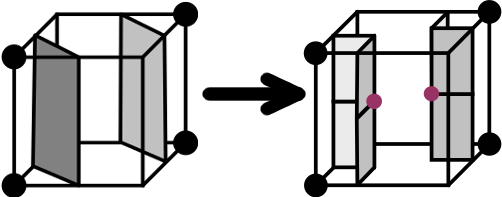
\includegraphics[width = .5\textwidth]{Pictures/SurfaceReconstruction/MCtoDualMC.png}
\end{center}
\caption{How one of the \ac{MC} cases is treaten in \ac{DualMC} algorithm (figure from \cite{Nielson2004})}
\end{figure}

\subsubsection{\acl{DualMT}}
While \ac{DualMC} is a very complicated algorithm, \acf{DualMT} uses tetrahedra instead of cubes and therefore reduces the $256$\footnote{With a proper treatment of ambiguities we get even more than those $256$ cases.} different cases from \ac{MC} to $2^4=16$ cases. Furthermore a treatment of ambiguous cases is not necessary anymore, since there are no ambiguous cases for this method\todointern{really? check this or find reference!}.
Even though the method is working on tetrahedra, we can still apply it to a voxel dataset, by composing each cube out of 5 or 6 tetrahedra (\autoref{fig:splittingCubes}). Nevertheless, this high amount of simplification comes with a drawback: The treatment of ambiguous cases depends on the splitting scheme applied to a cube\todointern{proof or reference! Show 2D example.}. Further detail on this method can be found in \cite{Nielson2008}.

\begin{figure}
\begin{center}
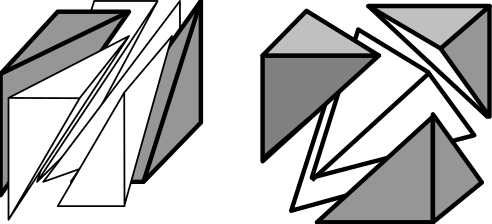
\includegraphics[width = .5 \textwidth]{Pictures/SurfaceReconstruction/SplittingCubes.png}
\caption{Two different subdivision schemes for cubes into tetrahedra (figure from \cite{Nielson2008})}
\label{fig:splittingCubes}
\end{center}
\end{figure}
